\documentclass{article}
\usepackage[utf8]{inputenc}
\usepackage[T1]{fontenc}
\usepackage[english]{babel}
\usepackage{graphicx}
\usepackage{tikz}
\usepackage{authblk}
\usepackage{enumitem}

\newcommand{\ls}[1]{\textcolor{red}{#1}}

% exemple papier seme https://hal.archives-ouvertes.fr/SEME
% https://hal.archives-ouvertes.fr/hal-01021660v1
% code GitHub : https://github.com/romainhild/pas   https://gitlab.math.unistra.fr/hild/pas


% thèse "Modélisation et évaluation de la performance des terminaux portuaires", Abderaouf Benghalia p 49
%https://tel.archives-ouvertes.fr/tel-01255291/document

%TODO: ???
% entête: seme, dates, labo, lieu
% en bas de page logos (cnrs, amies)

% demander autorisation PAS pour utiliser images 
% affiliations auteurs
% mise en page, voir https://hal.archives-ouvertes.fr/hal-01021660v1 ???

\title{\textbf{SEME in Strasbourg}\\[15pt] 
	Mathematical approaches to optimize the container positioning in the storage heart of the harbor terminals of the Port Autonome de Strasbourg}
\author[1]{Laurence Beaude} 
\author[2]{Céline Caldini-Queiros }
\author[2]{Romain Hild}
\author[2]{Mohamad Maassarani}
\author[2]{Myriam Maumy-Bertrand}
\author[2]{Lorenzo Sala}

\affil[1]{Universit\'e C\^ote d'Azur, CNRS, INRIA COFFEE, 
	Laboratoire J.A. Dieudonn\'e, 
	Parc Valrose, 06108 Nice cedex 02, France.} 
\affil[2]{Universit\'e de Strasbourg, IRMA, UMR 7501, 67000 Strasbourg, France.} 


\newcommand{\PAS}{\emph{Port Autonome de Strasbourg }}

\date{12-16 November 2018}




\begin{document}

\maketitle

\begin{center}
\textit{Topic proposed by:} \vspace{-3mm}
\begin{figure}[h!]
	\centering
	
\includegraphics[width=0.3\linewidth]{images/logo-pas}
\end{figure}
\end{center}

\noindent
\textbf{Abstract :} the goal of the SEME (Semaines d'\'Etude Mathématiques-Entreprises) consists in forming groups of young mathematical researchers that will work on a project proposed by a company for a whole week. \\
This report presents the work of one team that dealt with the problematic introduced by the \PAS (PAS).
Following the extension works in the south terminal of the harbor, the \PAS faced the issue how to optimize the placing of the container in their storage heart. \\
As first approach to the problem, we have considered just the stocking problem of the empty containers, due to the fact that these containers are the main part and they can stay longer in the terminal than the full ones.
Since the surface occupied by the empty containers is substantial and each container move is expensive, the storage has to be optimized in order to reduce the traveled kilometers and the operating costs. \\

\noindent
\textbf{Keywords :} Mathematical modeling , container storage.

\section{Introduction}

\ls{write something about the structure of the article ... }

\subsection{Background - state of the art}

The containerization was born in the early 50s by an American businessman, Malcom Purcell McLean.
He had the idea to transport commercial goods in big metal boxes, namely \textit{containers}.
From 1965, this containerization was promoted in every country for commercial transports overseas, however it was standardized only in 1974 by the ISO (International Standards Organization).
Since then the intermodal shipping via containers increased, which consists in using multiple way of traveling (boats, trains, trucks) for every good. \\
Nowadays, the river and sea transport has a crucial role in this globalized world.
Thus, for the last decades, the platforms for the intermodal exchange, including the \PAS, had to face the raise of the trans-shipment of containers between different way of transport. 
This new approach generates the issue of storing an increasing number of containers in the port terminals. 
Actually, when a container arrives, its exact position has to be decided in the yard of storage taking into account several constraints while ensuring the safety of the harbor site. 


\subsection{Glossary}
In this section we introduce the terminology we adopt in the following of the report. \\
\begin{itemize}[leftmargin=2.8cm]
	\item[\textbf{Reach-stacker.}] Vehicle that allows to move a container (see Fig. \ref{fig:pas_reach_stacker}).
	\item[\textbf{TEU.}] \textit{Twenty-foot Equivalent Unit},  measurement unit that corresponds to the length of small containers (see Fig. \ref{fig:teu}). 
	There are several types of containers that pass through the \PAS, including standard containers of 20 Feet (6.06mx 2.44mx 2.59m), 40 Feet (12.19mx 2.44mx 2.59m) or 40 Feet High Cube (12.19mx 2.35mx 2.90m ) and refrigerated containers of 20 or 40 feet.
	\item[\textbf{Position.}] Ground space where a container can be placed (see Fig. \ref{fig:name_definition}).
	\item [\textbf{Bay.}] Alignment of positions that are accessed by the same place (see Fig. \ref{fig:name_definition}). \\
	\item [\textbf{Heap.}] Stacking containers at one position (at most it's possible to stack 5 empty containers) (see Fig. \ref{fig:name_definition}). \\
	\item [\textbf{Block.}] Set of containers of a bay (see Fig. \ref{fig:name_definition}). \\
	\item [\textbf{Configuration.}] Storage plan with a precise distribution of positions and with a precise organization of customers among bays.
\end{itemize}

\begin{figure}[!htb]
	\begin{minipage}{0.45\linewidth}
		\centering
		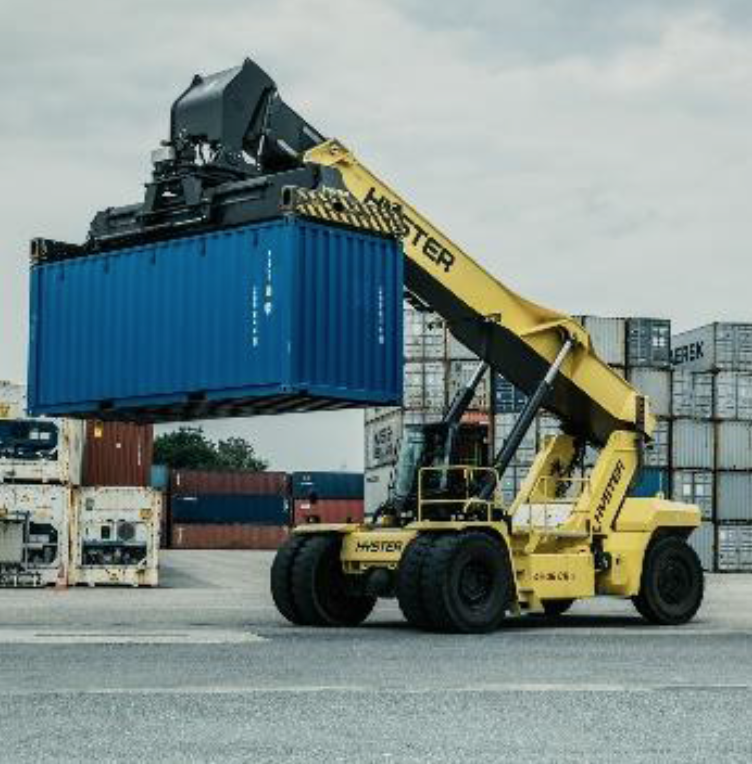
\includegraphics[width=0.8\linewidth]{images/PAS_stacker.png}
		\caption{Photo of a reach-stacker carrying a container.}
		\label{fig:pas_reach_stacker}
	\end{minipage}
	\begin{minipage}{0.55\linewidth}
		\centering
		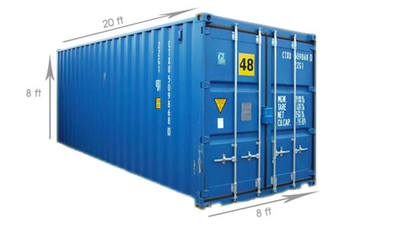
\includegraphics[width=\linewidth]{images/TEU.png}
		\caption{Dimensions of a container}
		\label{fig:teu}
	\end{minipage}
\end{figure}

\begin{figure}[h!]
	\centering
	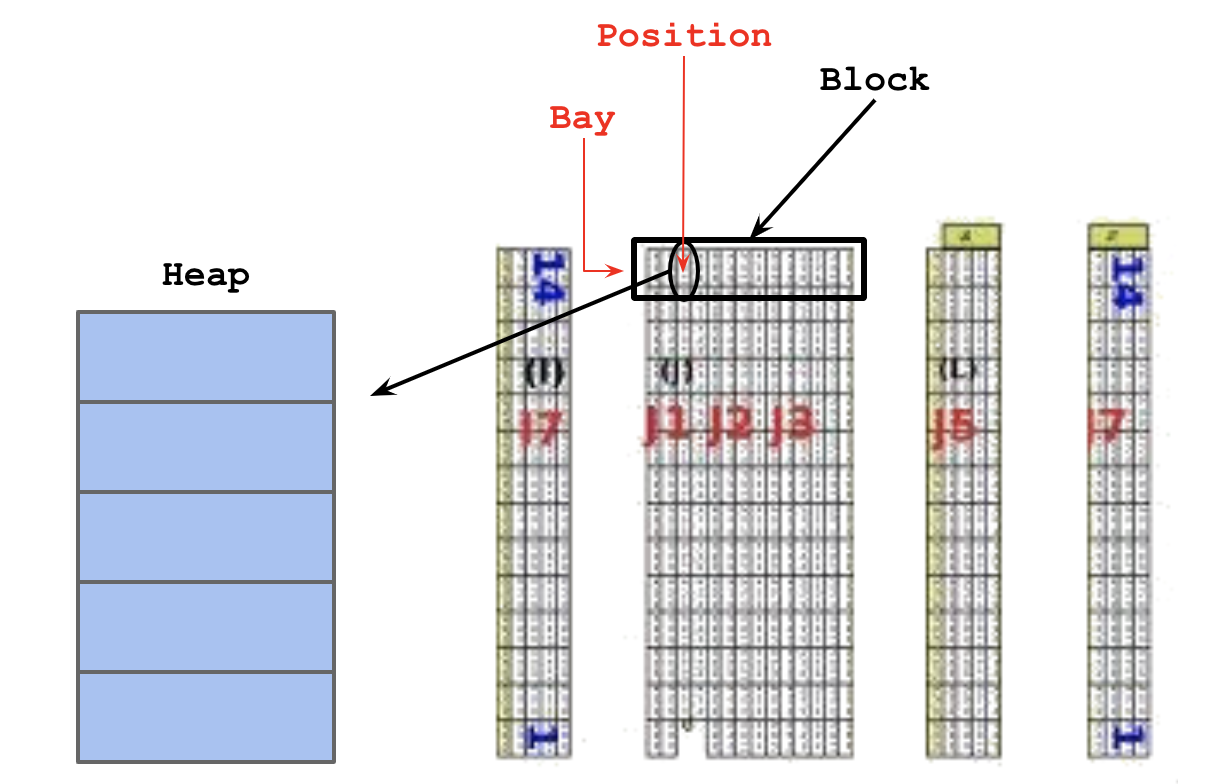
\includegraphics[width=0.8\linewidth]{images/glossary.png}
	\caption{Name definition for a storage area.}
	\label{fig:name_definition}
\end{figure}


\subsection{Presentation of the \PAS}

The \PAS is a multi-modal platform for the import/export of a wide variety of goods, It connects Strasbourg to seaports via the river and rail.
In 2017, $ 420000 $ TEU passed through this harbor and the $ 30 \% $ concerns the city. \\
The \PAS exploits two terminals, in our study we focus only the the South terminal. 
This terminal is transferring 20 feet or 40 feet containers between ferries and trucks, no rail transport is involved. 
It has two fluvial container cranes, one of which is mobile whereas the other is used to transport heavy packages, with a maximum capacity of $ 460 $ tonnes.
On average $3000$ empty containers are on the site with $500$ entries and $500$ exits every day counting all customers.



\begin{figure}[!htb]
\centering
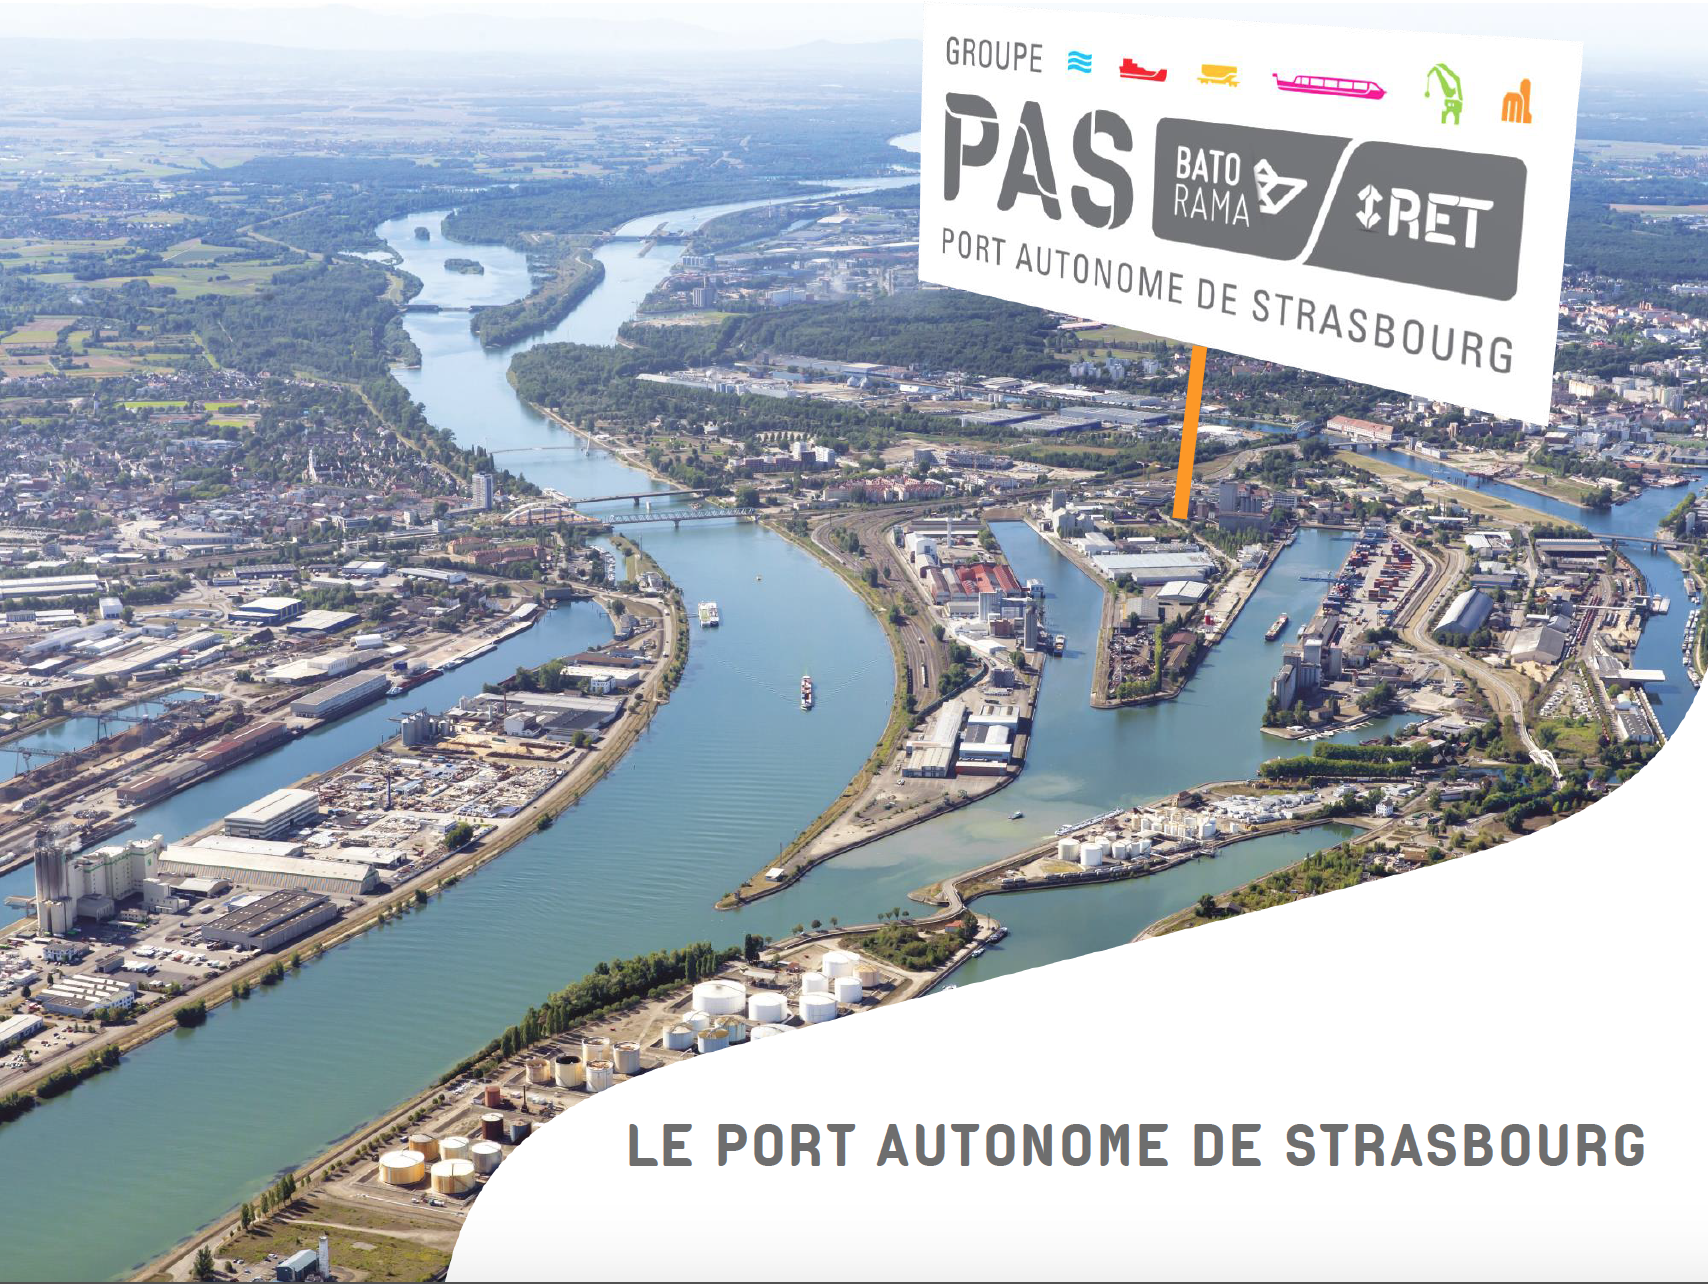
\includegraphics[width=0.7\linewidth]{images/PAS_satellite.png}
\caption{View of the North Terminal of the \PAS.}
\label{fig:pas_satellite}
\end{figure}

\subsection{\PAS issue}
This section summarizes the work done during the Week of Study \linebreak Mathematics-Business from 12 to 16 November 2018 in Strasbourg. \\
The \PAS has submitted a question related to the storage of empty containers in the harbor. 

Extension works will be done and the question of how to store, in the most effectively way, empty containers in the \PAS storage yard arises.
The problem is complex, because it depends on many parameters.
One of the main issue in developing a mathematical model in this context is the fact that the \PAS has no visibility on the date of release of the container when it enters their site. 

At this moment to optimize the storage, they have a software, which, when a container arrives, tells them where to deposit it.
This decision is based on the size of the container and the customer to whom it belongs. \\
This software can be configured to follow certain strategies and to respect fixed constraints but the choice of the positions on the ground where to store the containers is an input data and it has not been investigated in the past. \\
Therefore, our goal is to propose a storage plan and a customer distribution strategy for each bay in order to reduce the operating costs of the \PAS. 
This optimization has also a considerable impact in reducing congestion of trucks, shortening the handling time when they remain inactive.

In this early work we have considered the most important constraints that influence the storage system.
 
Firstly, each block must contain containers of \textbf{same dimensions} (three different container sizes pass through the \PAS) and \textbf{same client} (we neglect too small clients whose containers can to be mixed in one bay). 
Then, in order not to charge their customers too much, \PAS usually has a {First In, First Out} (FIFO) policy so that a particular container does not stay in the harbor too long. 
In fact, the daily price increases sharply when the container is stored after a certain number of days. 
This has an impact on the way the \PAS fills a block. 
Every block has to be accessible from both sides, because it is filled on one side and emptied by accessing it from the other aisle (see Figure \ref{fig: pas_config}). 
Thus, the first heap to be emptied is the oldest in the block. 


\begin{figure}[!htb]
\centering
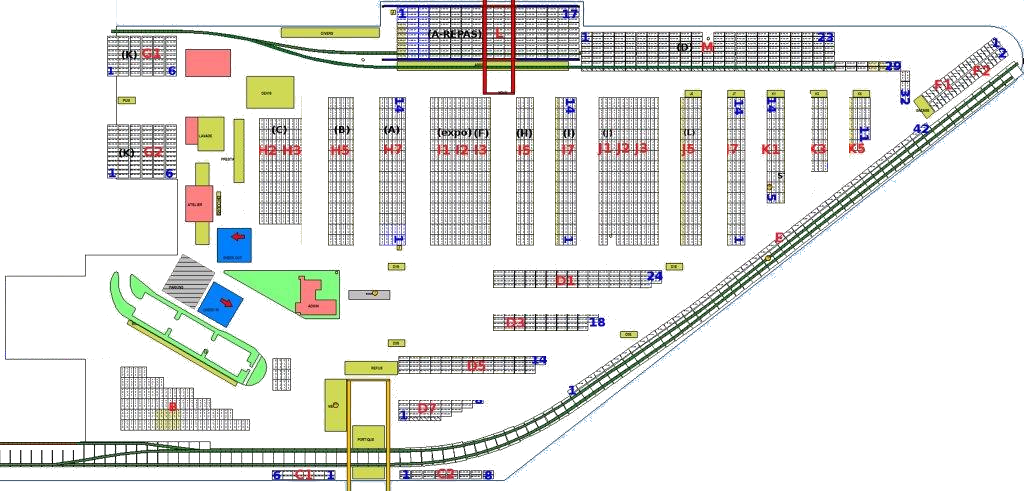
\includegraphics[width=\linewidth]{images/Plan_Terminal.png}
\caption{Current plan of the storage yard of the \PAS with the organization of the positions.}
\label{fig:pas_config}
\end{figure}




\section{Problem presentation and some possible solutions}

\textbf{Goal: find a configuration , which means find a distribution of positions on the storage area and an organization of customers in the defined areas, to minimize a cost function.} \\

\noindent
\textbf{Idea:} the representation of the height of the heaps has no impact in the problem because filling and emptying them is done automatically by bays that have the same container category (same dimensions and customer).
In addition, block management is managed by their computer system (TOS) and we have just to optimize the layout of the locations in the storage yard.
Thus, we have reduced the problem to a ground surface organization considering each bay independently. 
In other words, we have scaled down from a 3D problem where we had to consider the containers to a 2D problem of position distribution in the harbor.


\noindent
{\bf Issue: } draw the positions available in the harbor that can store $ 4500 $ TEU containers that belong to (???nb????) customers in order to minimize a cost function.


\subsection{State of the art} 
\ls{This part should be enhanced}

Several scientific works have been focused on the container storage optimization in the storage yard of port terminals. 
Firstly, we relied on the thesis entitled \textit{Algorithmes d'optimisation pour la résolution du problème de stockage de conteneurs dans un terminal portuaire} written by Ndèye Fatma Ndiaye in 2015 \cite{ndiaye2015}.
However, as our problem is a 2D position distribution problem in a harbor, we thought of several ways to approach this subject.

% https://www.researchgate.net/publication/294799315_Container_stacking_problem_a_survey

%Solution 1 : \\
%\indent
%- le problème revient à mailler la surface disponible dans le port avec des briques de taille 20*8pieds (petit conteneur), puis à repartir sur cette surface les travées (de tailles indiquées sur le plan) et les allées de circulations pour minimiser la distance. La meilleure configuration sera celle qui minimise la fonction coût définie ci-dessous.  \\

\begin{enumerate}[leftmargin=*,label=\emph{Solution \arabic*:}]
	\item draw inspiration from airport parking problems \cite{gotteland2004,deau2010optimisation}.
	\item shape optimization, level set (Yannick).
	\item combinatorial.
	\item heuristic.
	\item problem of distribution of 2D objects on a surface \cite{jacquenot2010}.
	\item see \cite{kim98}.
\end{enumerate}



\section{Several configurations comparison for the storage yard}

Due to lack of time - only few days of work - we decided to implement a C++ code that computes the cost function starting from specific configurations that we have previously drawn.
In this report we detail also some ideas for the automatic generation of storage plans.

\begin{figure}[!htb]
\centering
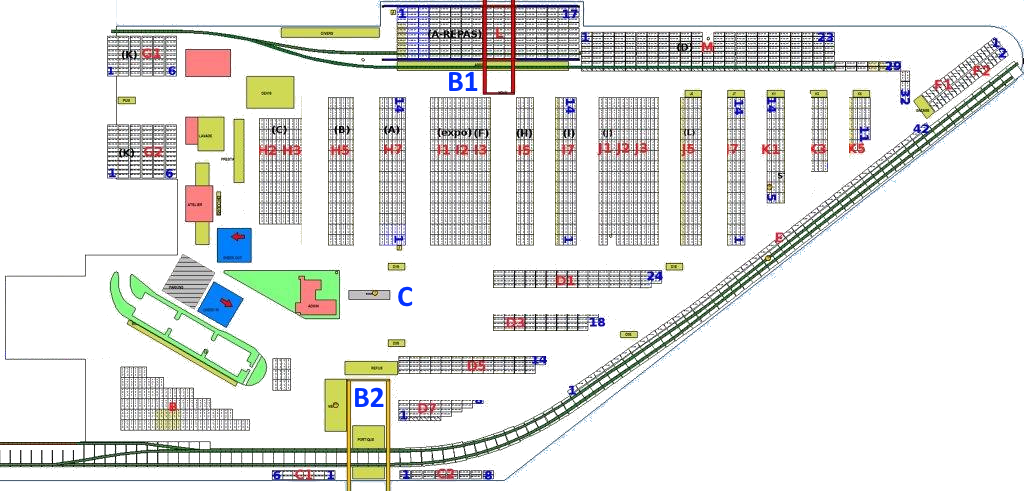
\includegraphics[width=\linewidth]{images/Plan_Terminal_modifie.png}
\caption{Current plan of the \PAS.}
\label{fig:pas_config_modif}
\end{figure}

Figure \ref{fig:pas_config_modif} shows the current plan of the \PAS, with the two fluvial cranes (B1 and B2) the the zone reserved for the truck loading/unloading (C). \\
The first complication is related to the unknown route of the containers because there are two fluvial portals. 
Therefore it is not possible to determine the exact distance because it is not known if the container will pass through the point B1 or B2.

Since we are focusing just on the empty containers, we have received the information that usually they arrive by boat (B1 or B2) and leave by truck (C).
By making this assumption, we know exactly the path, there is no uncertainty on the boat terminal because the container \underline{arrives} by this terminal. 
Hence the idea of cutting the area in two according to a symmetry that has to be determined and then optimize the two storage areas independently. 
Each zone would manage the empty containers arrived by its own boat terminal, which would always allow containers to be stored between the terminal and the truck loading/unloading area. \\

%-------------------------------------------------------%

Based on this hypothesis, we have simplified the problem by considering only the superior part of the \PAS (framed in the Figure \ref{fig:pas_config_encadre}).

\begin{figure}[!htb]
\centering
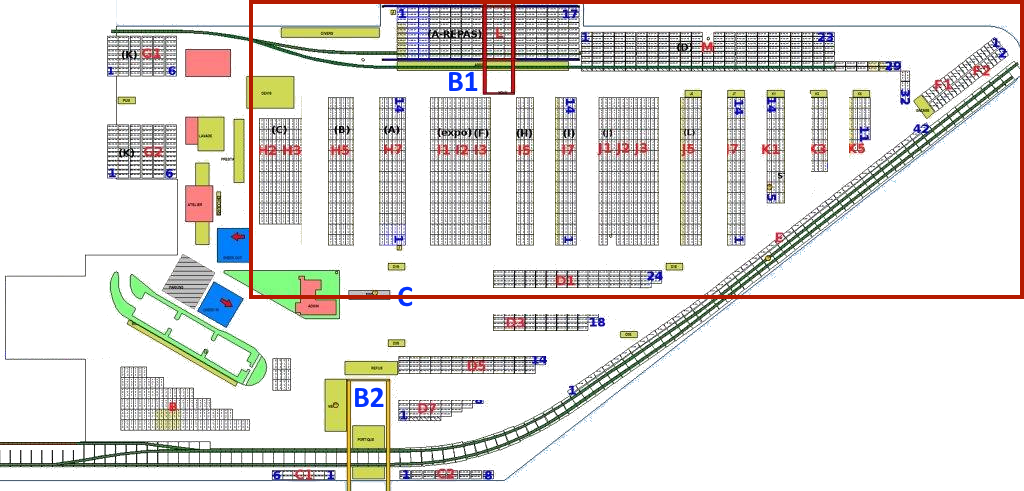
\includegraphics[width=\linewidth]{images/Plan_Terminal_encadre.png}
\caption{Zone of interest, sited between the boat terminal B1 et the truck loading/unloading area.}
\label{fig:pas_config_encadre}
\end{figure}

The number and position of the truck loading/unloading area can be modified.
An intuition is that this area should be at the (weighted) center of storage, however we are not taking into account the safety constraint to avoid the many crossings between trucks and reach-stackers. 
In addition, the truck must be accessible by the reach-stackers on both sides to put the container in the correct direction - the door must always be at the back -, which implies a empty zone of $15$ m on each side of the loading/unloading area. 
In this preliminary study we didn't complicate the configuration excessively, e.g. putting several loading/unloading areas, and we kept the point C fixed. \\
Figure \ref{fig:zone_reduced} illustrates the area on which we have conducted our study to optimize the storage (framed area in Figure \ref{fig:pas_config_encadre}).

\begin{figure}[!htb]
\centering
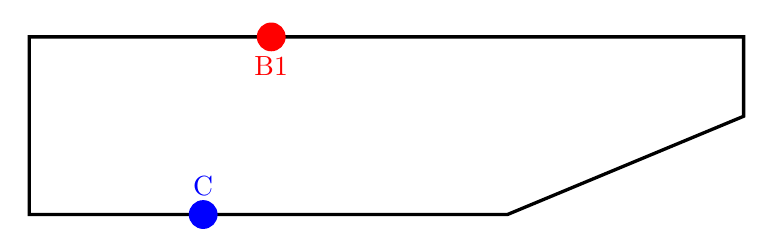
\begin{tikzpicture}[scale=0.06]
%\draw[help lines] (0,0) grid (142,-28);
\colorlet{Grey}{black!20}
%% External perimeter of the harbour
\draw[very thick] (0,0) -- (151.2,0)
	-- (151.2,-16.8) -- (151.2-50,-37.6)
	-- (0,-37.6) -- cycle;

%% Bateau
%\draw (46.4+4.8,0) circle[radius=5pt];
\node[mark size=5pt,color=red] at (46.4+4.8,0) {\pgfuseplotmark{*}};
\node[below,color=red] at (46.4+4.8,0-2) {B1};
%% Camion
\node[mark size=5pt,color=blue] at (4.8+32,-37.6) {\pgfuseplotmark{*}};
\node[above,color=blue] at (4.8+32,-37.6+2) {C};
\end{tikzpicture}
\caption{Reduced area of the \PAS on which we have focused.}
\label{fig:zone_reduced} 
\end{figure}




\subsection{Definition of the cost function}

To compare different configurations,we need to define a cost function that evaluates their performance. \\ 
\underline{Reminder}: a configuration is defined by a plan of positions and a distribution of the customers among the bays. 


The cost function estimates the costs of moving a fixed number of containers that are present in the harbor on average. 
This cost function takes into account the input/output movements of each container according to a weight that depends on each customer.
This weight represents the frequency of movement of a container, indeed, we assume that each client asks with regularity to obtain or store a container, and, thanks to the FIFO policy, every container of the same customer is moved with the same frequency. 


For each client, we set a \textbf {volume} that represents the number of containers stored in the port on average and a \textbf {weight} that is calculated based on the frequency of the movements. 
This process helps in the understanding  the distribution of customers once a position plan has been drawn. 
For example, a customer with few containers and a lot of movement (entry or exit of containers) would likely have a short bay and it should have a computed short distance; a client who stores large volumes and moves a lot may have longer bays (or many small bays) and again the computed distance should be low; a customer with few movements can be stored further away regardless of the volume. \\

\noindent
\textbf{Notations:} 

\begin{table}[!htb]
\centering
 \begin{tabular}{|c|l|}
\hline
$t$ & bay index \\[3pt]
$c$ & client index \\[3pt]
$N_t$ & length of the bay $t$ \\[3pt]
$V_c$ & number of containers stacked in the harbor that belong to client $c$ \\[3pt]
$V_{tot}$ & total number of containers \\[3pt]
$d_t$ & distance that has to be traveled from the crane to the bay and \\
& from the bay to the truck loading area \\[3pt]
$\mu_c$ & weight that represents the frequency of the movements of containers \\ 
& that belong to client $c$ \\[3pt]
$x_{t,c}$ & number of positions used by client $c$ in the bay $t$ \\[3pt]
\hline
\end{tabular}
\end{table}

\paragraph{Cost function:}

% sum   distance * probabilité que la pile bouge
\begin{equation}
\displaystyle \sum_t \sum_c (d_t \,\, \mu_c \,\, x_{t,c})
\end{equation}



Following the hypothesis proposed by the company, to be able to draw possible layouts for the containers position and the distribution of customers in a realistic way, we have imposed also the following constraints:
\begin{itemize}
	\item traffic lanes must be at least $15$ m wide;
	\item the reach-stacker has to access a bay by its width to catch the container on the side;
	\item every containers belongs to a client, whether $$\sum_ {c} V_c = V_ {tot} $$;
	\item in each bay $ t $, there are no more positions used than the one available, whether $$0\le \sum_c x_{t,c} \le N_t$$;
	\item containers of different client cannot be in the same bay $t$, whether \linebreak $$x_{t,c}*x_{t,c'}=0, \,\,\, \forall c \neq c'$$.
\end{itemize}

\subsection{Study on different configurations} 

The definition of the test case should not be done casually because the optimal storage plan obtained depends very much on our choice. 
For instance, the total volume of containers stored on the site, their distribution by customer and each customer frequency have a strong impact on the optimal storage plan. 

\ls{Do we have to show more test cases?}

Following the information we have received from \PAS, the empty containers of any dimensions that are stocked in the storage yard are $3000$ on average.
For simplicity we consider $V_{tot}=4500$ TEU. 

To define the weights $ \ mu_c $ associated to each customer frequency of movement, we have exploited the data on the movements of September and October 2018 given directly by the \PAS.
 
 \ls{write the formula to compute these weights}

%$
%\mu_c = \frac{\sum_{} mvt du client c}{mvt totaux} 
%$

\begin{figure}[!htb]
\centering
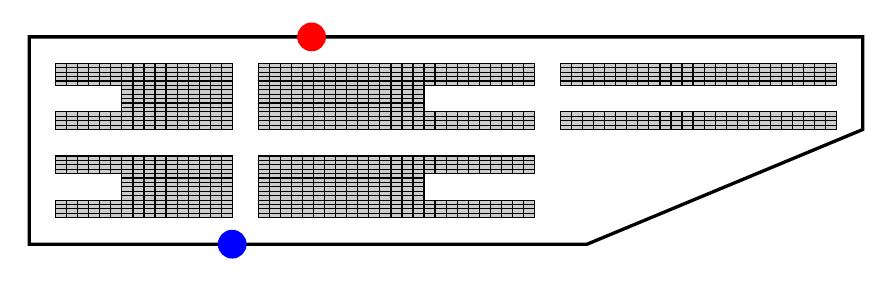
\begin{tikzpicture}[scale=0.07]
%\draw[help lines] (0,0) grid (142,-28);
\colorlet{Grey}{black!20}
%% External perimeter of the harbour
\draw[very thick] (0,0) -- (151.2,0)
	-- (151.2,-16.8) -- (151.2-50,-37.6)
	-- (0,-37.6) -- cycle;
%% Zone top left
\def\a{4.8}
\def\b{-4.8}
\draw[fill=Grey] (\a,\b) -- (\a+32,\b)
	-- (\a+32,\b-12) -- (\a,\b-12)
	-- (\a,\b-12+3.2) -- (\a+12,\b-12+3.2)
	-- (\a+12,\b-4) -- (\a,\b-4) -- cycle;
%
\foreach \x in {0,...,5}
{
	\draw[thin] (\a+2*\x,\b) -- (\a+2*\x,\b-0.8*5);
	\draw[thin] (\a+2*\x,\b-12) -- (\a+2*\x,\b-12+0.8*4);
	\draw[thin] (\a,\b-0.8*\x) -- (\a+32,\b-0.8*\x);
}
\foreach \x in {0,...,10}
{
	\draw[thin] (\a+12+2*\x,\b) -- (\a++12+2*\x,\b-0.8*15);
}
\foreach \x in {0,...,4}
	{\draw[thin] (\a,\b-4-4.8-0.8*\x) -- (\a+32,\b-4-4.8-0.8*\x);}
\foreach \x in {0,...,6}
	{\draw[thin] (\a+12,\b-4-0.8*\x) -- (\a+32,\b-4-0.8*\x);}
%%%%%%%%%%%%%%		
%% Zone bottom left %%
%%%%%%%%%%%%%%
\def\a{4.8}
\def\b{-21.6}
\draw[fill=Grey] (\a,\b) -- (\a+32,\b)
-- (\a+32,\b-11.2) -- (\a,\b-11.2)
-- (\a,\b-11.2+3.2) -- (\a+12,\b-11.2+3.2)
-- (\a+12,\b-3.2) -- (\a,\b-3.2) -- cycle;
%
\foreach \x in {0,...,5}
{
	\draw[thin] (\a+2*\x,\b) -- (\a+2*\x,\b-0.8*4);
	\draw[thin] (\a+2*\x,\b-11.2) -- (\a+2*\x,\b-11.2+0.8*4);
}
\foreach \x in {0,...,10}
{
	\draw[thin] (\a+12+2*\x,\b) -- (\a+12+2*\x,\b-0.8*14);
}
\foreach \x in {0,...,4}
{
	\draw[thin] (\a,\b-3.2-4.8-0.8*\x) -- (\a+32,\b-3.2-4.8-0.8*\x);
	\draw[thin] (\a,\b-0.8*\x) -- (\a+32,\b-0.8*\x);
}
\foreach \x in {0,...,6}
	{\draw[thin] (\a+12,\b-3.2-0.8*\x) -- (\a+32,\b-3.2-0.8*\x);}
%%%%%%%%%%%%%%
%% Zone top central %%
%%%%%%%%%%%%%%
\def\a{41.6}
\def\b{-4.8}
\draw[fill=Grey] (\a,\b) -- (\a+50,\b)
	-- (\a+50,\b-4) -- (\a+50-20,\b-4)
	-- (\a+50-20,\b-4-4.8) -- (\a+50,\b-4-4.8)
	-- (\a+50,\b-12) -- (\a,\b-12) -- cycle;
%
\foreach \x in {0,...,15}
{
	\draw[thin] (\a+2*\x,\b) -- (\a+2*\x,\b-0.8*15);
	\draw[thin] (\a,\b-0.8*\x) -- (\a+30,\b-0.8*\x);
}
\foreach \x in {0,...,10}
{
	\draw[thin] (\a+30+2*\x,\b) -- (\a+30+2*\x,\b-0.8*5);
	\draw[thin] (\a+30+2*\x,\b-8.8) -- (\a+30+2*\x,\b-8.8-0.8*4);
}
\foreach \x in {0,...,5} {\draw[thin] (\a+30,\b-0.8*\x) -- (\a+50,\b-0.8*\x);}
\foreach \x in {0,...,4} {\draw[thin] (\a+30,\b-8.8-0.8*\x) -- (\a+50,\b-8.8-0.8*\x);}
%%%%%%%%%%%%%%%%
%% Zone bottom central %%
%%%%%%%%%%%%%%%%
\def\a{41.6}
\def\b{-21.6}
\draw[fill=Grey] (\a,\b) -- (\a+50,\b)
-- (\a+50,\b-3.2) -- (\a+50-20,\b-3.2)
-- (\a+50-20,\b-3.2-4.8) -- (\a+50,\b-3.2-4.8)
-- (\a+50,\b-11.2) -- (\a,\b-11.2) -- cycle;
%
\foreach \x in {0,...,4} {
	\draw[thin] (\a+30,\b-0.8*\x) -- (\a+50,\b-0.8*\x);
	\draw[thin] (\a+30,\b-8-0.8*\x) -- (\a+50,\b-8-0.8*\x);
}
\foreach \x in {0,...,10}
{
	\draw[thin] (\a+30+2*\x,\b) -- (\a+30+2*\x,\b-0.8*4);
	\draw[thin] (\a+30+2*\x,\b-8) -- (\a+30+2*\x,\b-8-0.8*4);
}
\foreach \x in {0,...,15} {\draw[thin] (\a+2*\x,\b) -- (\a+2*\x,\b-0.8*14);}
\foreach \x in {0,...,14} {	\draw[thin] (\a,\b-0.8*\x) -- (\a+30,\b-0.8*\x);}
%%%%%%%%%%%%%%%%
%%%% Zone top right %%%%
%%%%%%%%%%%%%%%%
\def\a{41.6+4.8+50}
\def\b{-4.8}
\draw[fill=Grey] (\a,\b) -- (\a+50,\b)
-- (\a+50,\b-4) -- (\a,\b-4) -- cycle;
\draw[fill=Grey] (\a,\b-4-4.8) -- (\a+50,\b-4-4.8) 
	-- (\a+50,\b-4-4.8) -- (\a+50,\b-12) -- (\a,\b-12) -- cycle;
%
\foreach \x in {0,...,25} {
	\draw[thin] (\a+2*\x,\b) -- (\a+2*\x,\b-0.8*5);
	\draw[thin] (\a+2*\x,\b-8.8) -- (\a+2*\x,\b-8.8-0.8*4);
}
\foreach \x in {0,...,5} {\draw[thin] (\a,\b-0.8*\x) -- (\a+50,\b-0.8*\x);}
\foreach \x in {0,...,4} {\draw[thin] (\a,\b-8.8-0.8*\x) -- (\a+50,\b-8.8-0.8*\x);}
%% Bateau
%\draw (46.4+4.8,0) circle[radius=5pt];
\node[mark size=5pt,color=red] at (46.4+4.8,0) {\pgfuseplotmark{*}};
%% Camion
\node[mark size=5pt,color=blue] at (4.8+32,-37.6) {\pgfuseplotmark{*}};
\end{tikzpicture}
\caption{Another possible configuration/}
\label{fig:2D_PAS_actuel} 
\end{figure}

\ls{write the results!}

\section{Next steps: automatic generation of configurations} 

In this section we introduce two ideas for an algorithm to generate a large number of possible configurations.
In a second step we can compute the cost function on these generated configurations in order to select the best one.

\paragraph{Creating plans with $ n $ horizontal and $ m $ vertical aisles.} 
This algorithm defines the place of the aisles varying $ n $ and $ m $. 
In this way it is possible to quickly create configuration but with the strong constraint that all the aisles are oriented horizontally or vertically. 
For a possible implementation we recommend that the aisles may not cross the entire surface each time.

\paragraph{Creation of plans with a snake algorithm.}
This algorithm consists in creating paths from a starting point (e.g. one of the cranes). % biblio ???

\noindent
\textit{Initialization:}
\begin{itemize}
	\item mesh the plan of the \PAS with a grid size equal to the dimension of the smallest container. Each mesh element is called pixel in the following. We denote $ (dx, dy) $ the size of the mesh;
	\item every pixel is either a traffic aisle ($ a $), or a container position ($ e $);
	\item define a minimum number of positions ($N_e=4500$). 
\end{itemize}

\noindent
\textit{Algorithm:}
\begin{itemize}
	\item initialize all pixels to $ e $ (these are container positions), and initialize the position of the snake on the pier $ (x_0, y_0) = (x_ {ship}, y_ {ship}) $;

    \item  loop till $\#e>N_e$ whether the number of positions is sufficiently big:
    \begin{enumerate}
        \item\label{next_position} the snake moves to the position $(x_{i+1},y_{i+1})$ with the following rules
			\begin{eqnarray}
			x_{i+1} = \left\{\begin{array}{l}
			x_i, \\
			x_i + dx,\\
			x_i + dx, \\
			\end{array}\right. \qquad
			y_{i+1}	 = \left\{\begin{array}{l}
			y_i, \\
			y_i + dy,\\
			y_i + dy. \\
			\end{array}\right.
			\nonumber
			\end{eqnarray};
			 \item  loop with a snail shape around $(x_{i+1},y_{i+1})$ to define the aisle $a$ every pixel which distance from $(x_{i+1},y_{i+1})$ is fewer than $15$m; % $15+\sqrt{(dx^2+dy^2)}/2$m ($\sqrt{(dx^2+dy^2)}/2$ car la distance est calculée avec le centre de la maille alors que le reach-stacker ne doit pas taper dans les coins du conteneur), 
			\item  update the number of container positions $\#e$.
	\end{enumerate}
	\item check that the configuration obtained complies with the constraints, including that the truck loading/unloading area belongs to a path, and then compute the cost function on this new configuration.
\end{itemize}

It may be interesting to constrain the algorithm to choose certain possibilities for the position $ (x_ {i + 1}, y_ {i + 1}) $ with a greater probability. 
For example, in our case it seems logical to favor a straight line and avoid too many bends. 
Thus, instead of choosing with the same probability each direction, the step \ref{next_position} can be adapted to prefer the straight line.


\section{Discussion on FIFO}
One of the hypotheses that strongly constrains storage geometry is related to  the logic \textit{First In, First Out}. 
Indeed, this fact implies that the stack-reacher has to access to the containers by the two sides of the bay, imposing that the optimization of the bay length is strongly influenced by the to the volume and the frequency of movements of each customer. 
The logic FIFO adopted by the \PAS is due to the fact that the client would like to access every time to the oldest container of each bay since the billing depends on how long each container is stored in the harbor. \\
As alternative we propose the logic \textit{Last In, First Out} (LIFO), indeed this storage management would greatly reduce the areas allocated to the traffic aisles and would make it possible to pick up the containers that require the least total distance (from the harbor to the truck loading area). 
This alternative idea raised during the week would be integrated with the previous billing strategy, namely we suggest a FIFO invoicing management coupled with a LIFO logic for the storage.


\section{Conclusion}

\ls{write conclusions}

%%%%%%%%%

\bibliographystyle{plain}
\bibliography{biblio}

\end{document}
